\section{Meta-heuristic optimisation of the charging station placement}
\label{sec:7_7a_opt}

In section \mc{indicare sezione},  I pointed out how \textit{Num Parking} placement heuristic works better than the other two.
Weighting also charges and re-routing, the \textit{Hybrid} policy shows better performances than \textit{Needed}. For this reason, in this section, I focus on the \textit{Hybrid} return policy with charging stations covering less than 15\% of the zones. I further optimise this scenario by running the meta-heuristic placement algorithms, and comparing the results with the \textit{Num Parking} placement. 
Optimisation with \textit{Needed} return policies are briefly discussed in \ref{sec:7_7b_needed}, where very similar results are obtained.  


The hill-climbing local search, here abbreviated in \textit{Local Search}, uses \textit{Num Parking} placement as initial solution. The \textit{Genetic} algorithm creates a totally new solution without exploiting any previous knowledge. 
Recall that both algorithms are designed to find the best charging stations placement that guarantee 0 infeasibile trips, and to minimise the overall distance the customer has to walk to reach the final destination.


\begin{figure}[th]
    \centering     %%% not \center
    \subfloat[][Percentage of infeasible trips.  Y-Axis is logarithmic.]
    {
      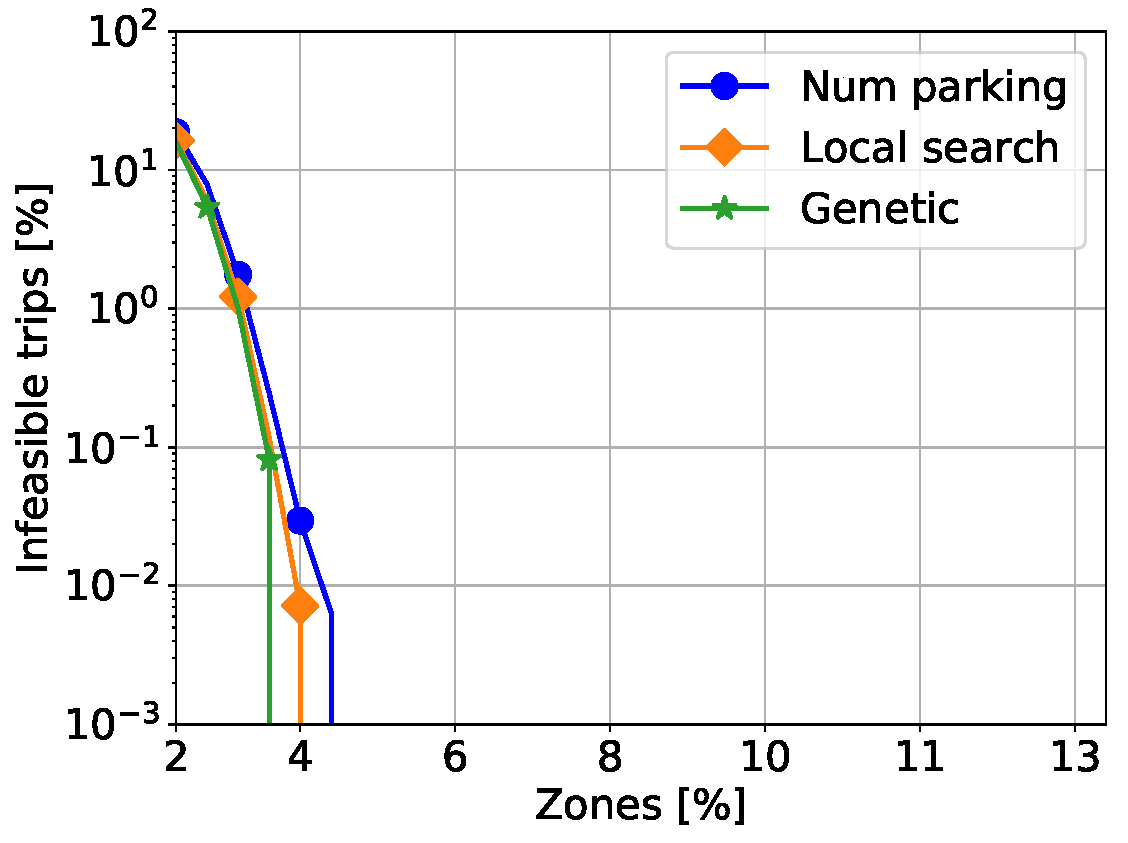
\includegraphics[width=0.45\textwidth]{figures/Hybrid_Deaths.pdf}
        \label{fig:7_7a_optimized_deaths}
    }
    \subfloat[][Average walked distance.]
    {
        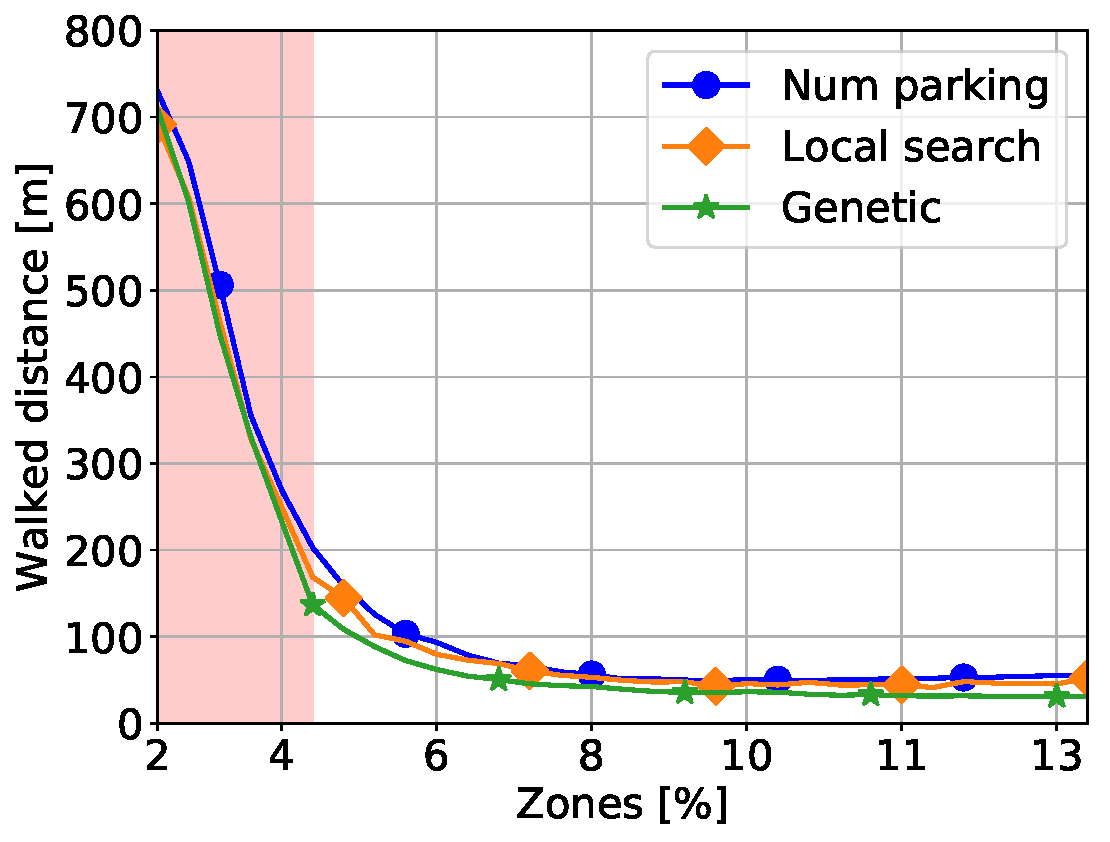
\includegraphics[width=0.45\textwidth]{figures/Hybrid_TravelWithPenlaty.pdf}
        \label{fig:7_7a_optimized_penaly}
    }    
    \label{fig:7_7a_optimized_metrics}
    \caption{Objective metrics to minimise in the optimisation - with \textit{Hybrid} return policy.}
\end{figure}

\begin{figure*}[t!]
	\begin{center}
		\begin{subfigure}{0.49\textwidth}
			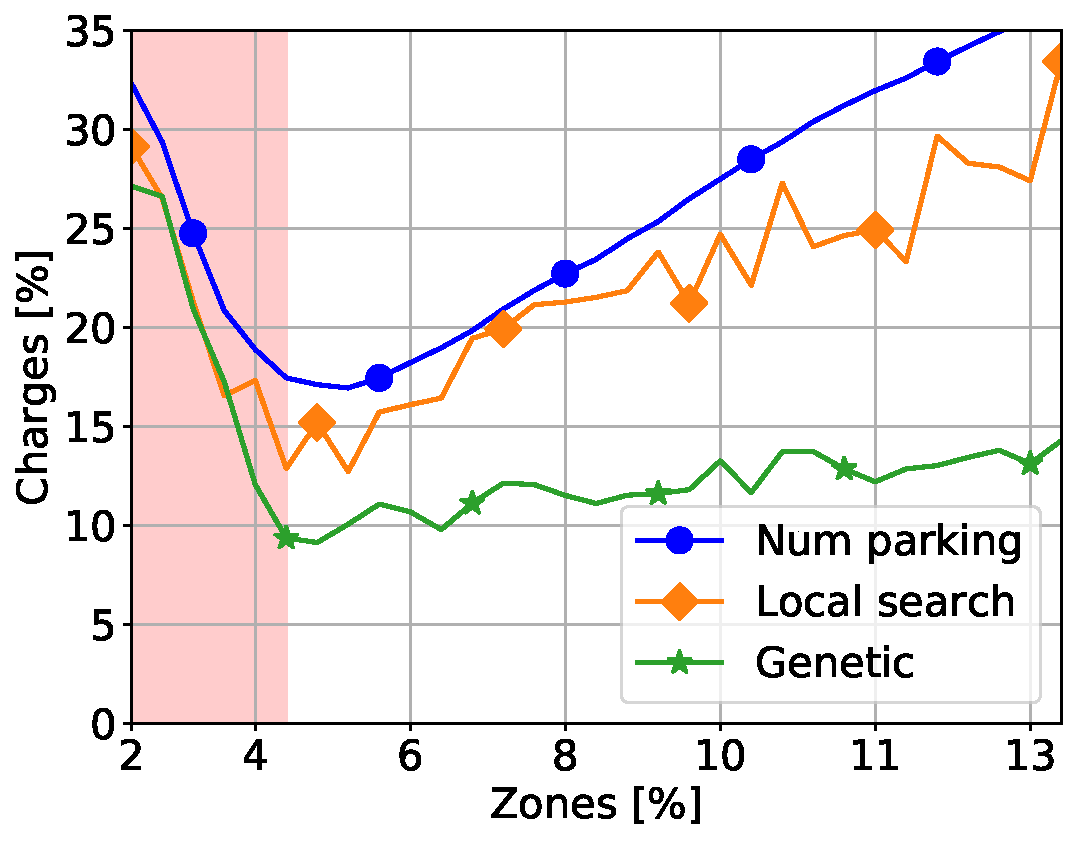
\includegraphics[width=\columnwidth]{figures/Hybrid_AmountRechargePerc.pdf}
			\caption{Average state of charge.}
			\label{fig:7_7a_recharge}
		\end{subfigure}
		\begin{subfigure}{0.49\textwidth}
			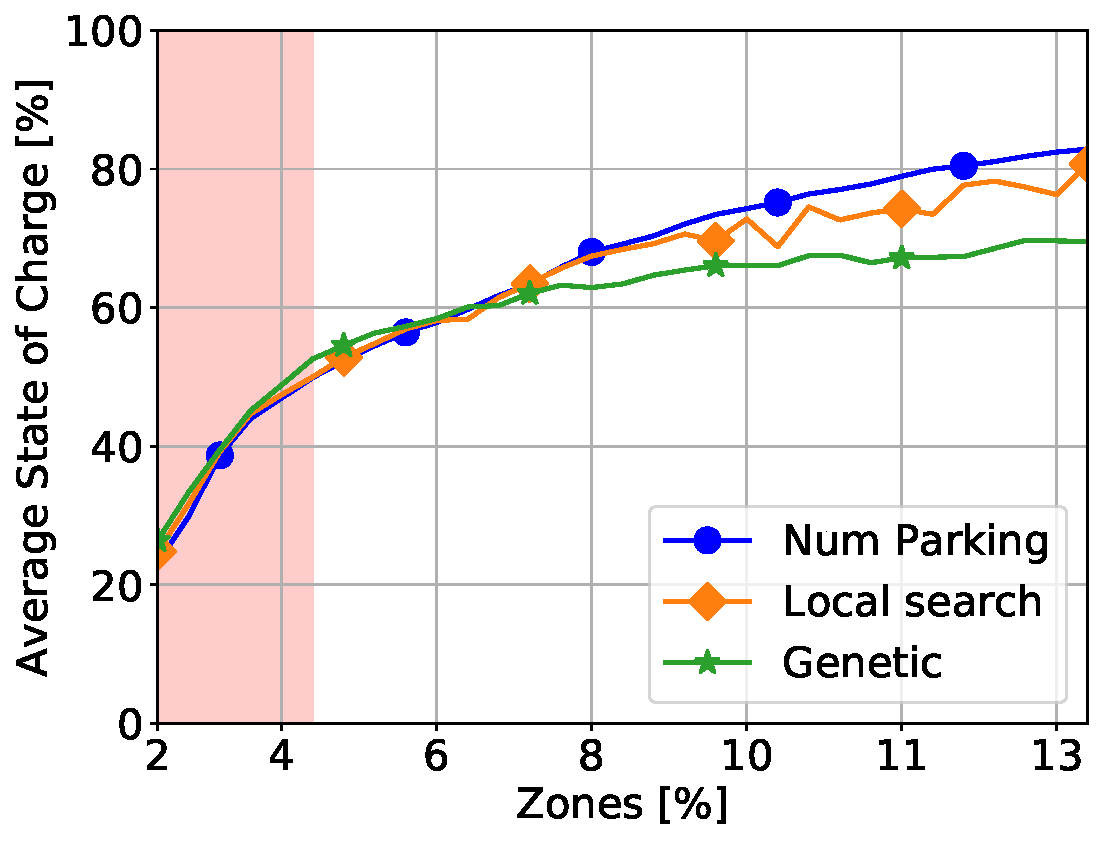
\includegraphics[width=\columnwidth]{figures/AvgSOC_comparison}
			\caption{Average state of charge.}
			\label{fig:7_7a_asoc_Needed}
		\end{subfigure}
	
		\begin{subfigure}{0.49\textwidth}
			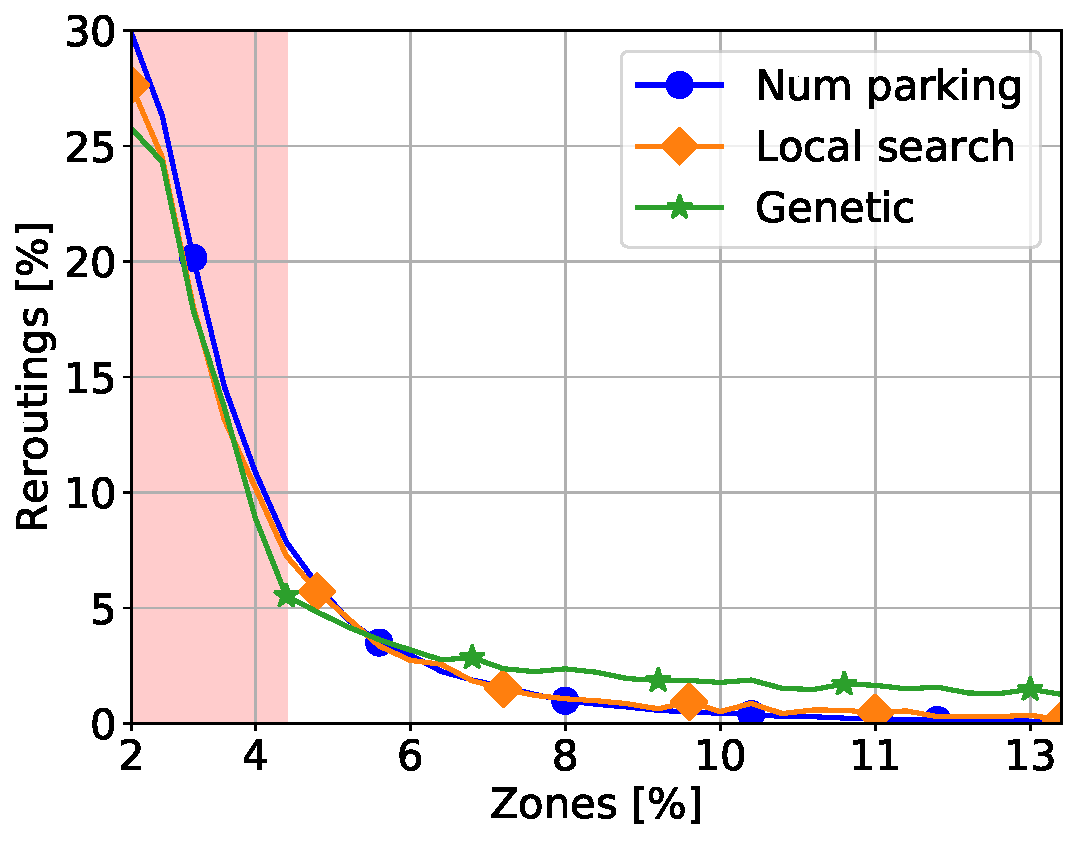
\includegraphics[width=\columnwidth]{figures/Hybrid_ReroutePerc.pdf}
			\caption{Rerouted trips percentage.}
			\label{fig:7_7a_reroute}
		\end{subfigure}
		\begin{subfigure}{0.49\textwidth}
			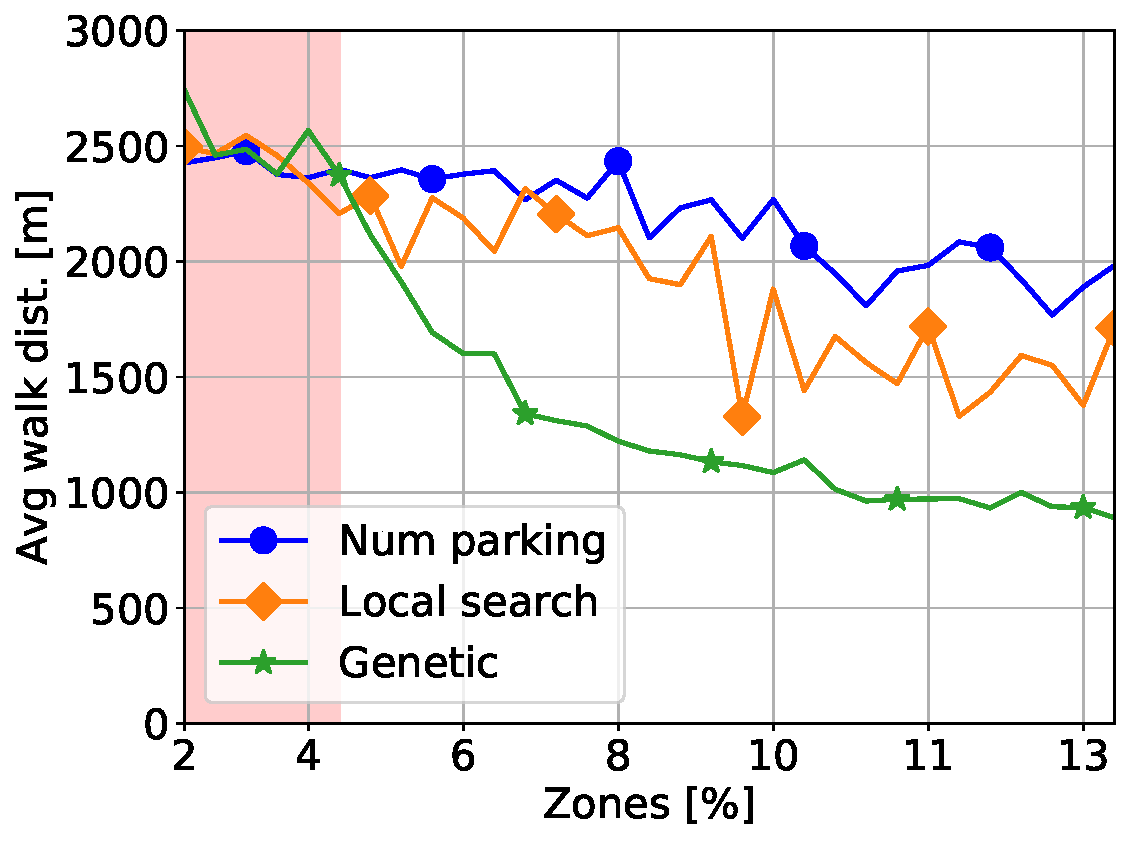
\includegraphics[width=\columnwidth]{figures/Hybrid_AvgWalkedDistance.pdf}
			\caption{Rerouted trips percentage.}
			\label{fig:7_7a_awd}
		\end{subfigure}         
    \caption{\textit{Genetic} and \textit{Local Search} optimisation results for metrics of interests (\textit{Hybrid} return policy adopted).}
	\label{fig:7_7a_hybrid_optimization}
	\end{center}
\end{figure*}


Figure.~\ref{fig:7_7a_optimized_metrics} reports the two target metrics, for all the optimised configurations.
Firstly, in figure.~\ref{fig:7_7a_optimized_deaths} I compare the infeasible trip percentage. \textit{Num Parking} solution (blue line) has already good performance, reaching 0 with 4.2\% of the equipped zones. 
The \textit{Local Search} (orange line) and the \textit{Genetic} (green line) algorithms are able to further reduce the minimum percentage of zone to equip to guarantee no infeasible trips: 3.8\% by the \textit{Local Search}, and to 3.5\% with the \textit{Genetic} algorithm, $Z=10$ and $Z=9$ zones respectively.


Figure.~\ref{fig:7_7a_optimized_penaly} reports the walked distance. Focusing in the feasible region, the \textit{Genetic} algorithm confirms the best performance, reducing the distance from more than 200\,m to 136\,m when 4.2\% of the zones are equipped with charging stations, and reaching just 30\,m at 13\%. 


In figure.~\ref{fig:7_7a_hybrid_optimization} I further study the new solutions on other metrics.
Figure \ref{fig:7_7a_recharge} reports the percentage of trips ending in a charging station. The more charges are performed, the more time the customer has to spend time plugging/unplugging the car. By minimising the walked distance, I also reduce this metric, since a trip ending with a charge corresponds to 150\,m of penalty.
Here, the \textit{Local Search} follows the same trend as the \textit{Num parking} with a strong rise. The \textit{Genetic} algorithm shows much better results, from 9\% to 14\% of trips ending with a charge -- half of those found with other solutions. 
This improvement highlights the better placement of the charging stations.
Focus now on figure. \ref{fig:7_7a_asoc}, which reports the average state of charge of the car battery. 
No major difference are observed here, with all curves almost overlapping up to 7\% of the zones.

In a nutshell, the solution found by the \textit{Genetic} algorithm lets customers charge much less frequently, while keeping the average state of charge very similar. Consider next figure \ref{fig:7_7a_reroute}, which details the percentage of reroutes. It is possible to see how the trend is the opposite with respect to the previous ones. Here, the \textit{Genetic} optimised solution show a little higher re-routing percentage than the \textit{Num parking}. In particular, the \textit{Genetic} algorithm reaches 1.3\% of reroutes, while \textit{Num parking} decreases down to 0.2\% of reroutes. Indeed, the \textit{Genetic} algorithm places charging stations not only where most rentals ends, but also so to decrease the customers' average walked distance, i.e., in those places where likely cars are not so frequently parked but that can be quickly reached in case of re-routing.
To understand the importance of this difference, in figure~\ref{fig:7_7a_awd} I evaluate the walking distance a customer has to walk because she suffered a reroute.  
The \textit{Genetic} algorithm is able to push the walked distance below 1\,km, while the \textit{Local Search} generates marginal improvements.
In a nutshell, despite customers are rerouted more frequently, on average, they walk for a shorter, and  more bearable, distance.


In conclusion, a smart placement of the charging stations is better under different perspectives.  The \textit{Genetic} solution, tailored on the data of the usage behaviour, allows us to improve both the system performance, and customers' discomfort, in particular by greatly reducing the number of times they have to charge, and the distance they have to walk.


\subsection{Charging station placement visualisation}

\begin{figure}[h!]
    \centering     %%% not \center
    \subfloat[][Number of Parkings.]
    {
        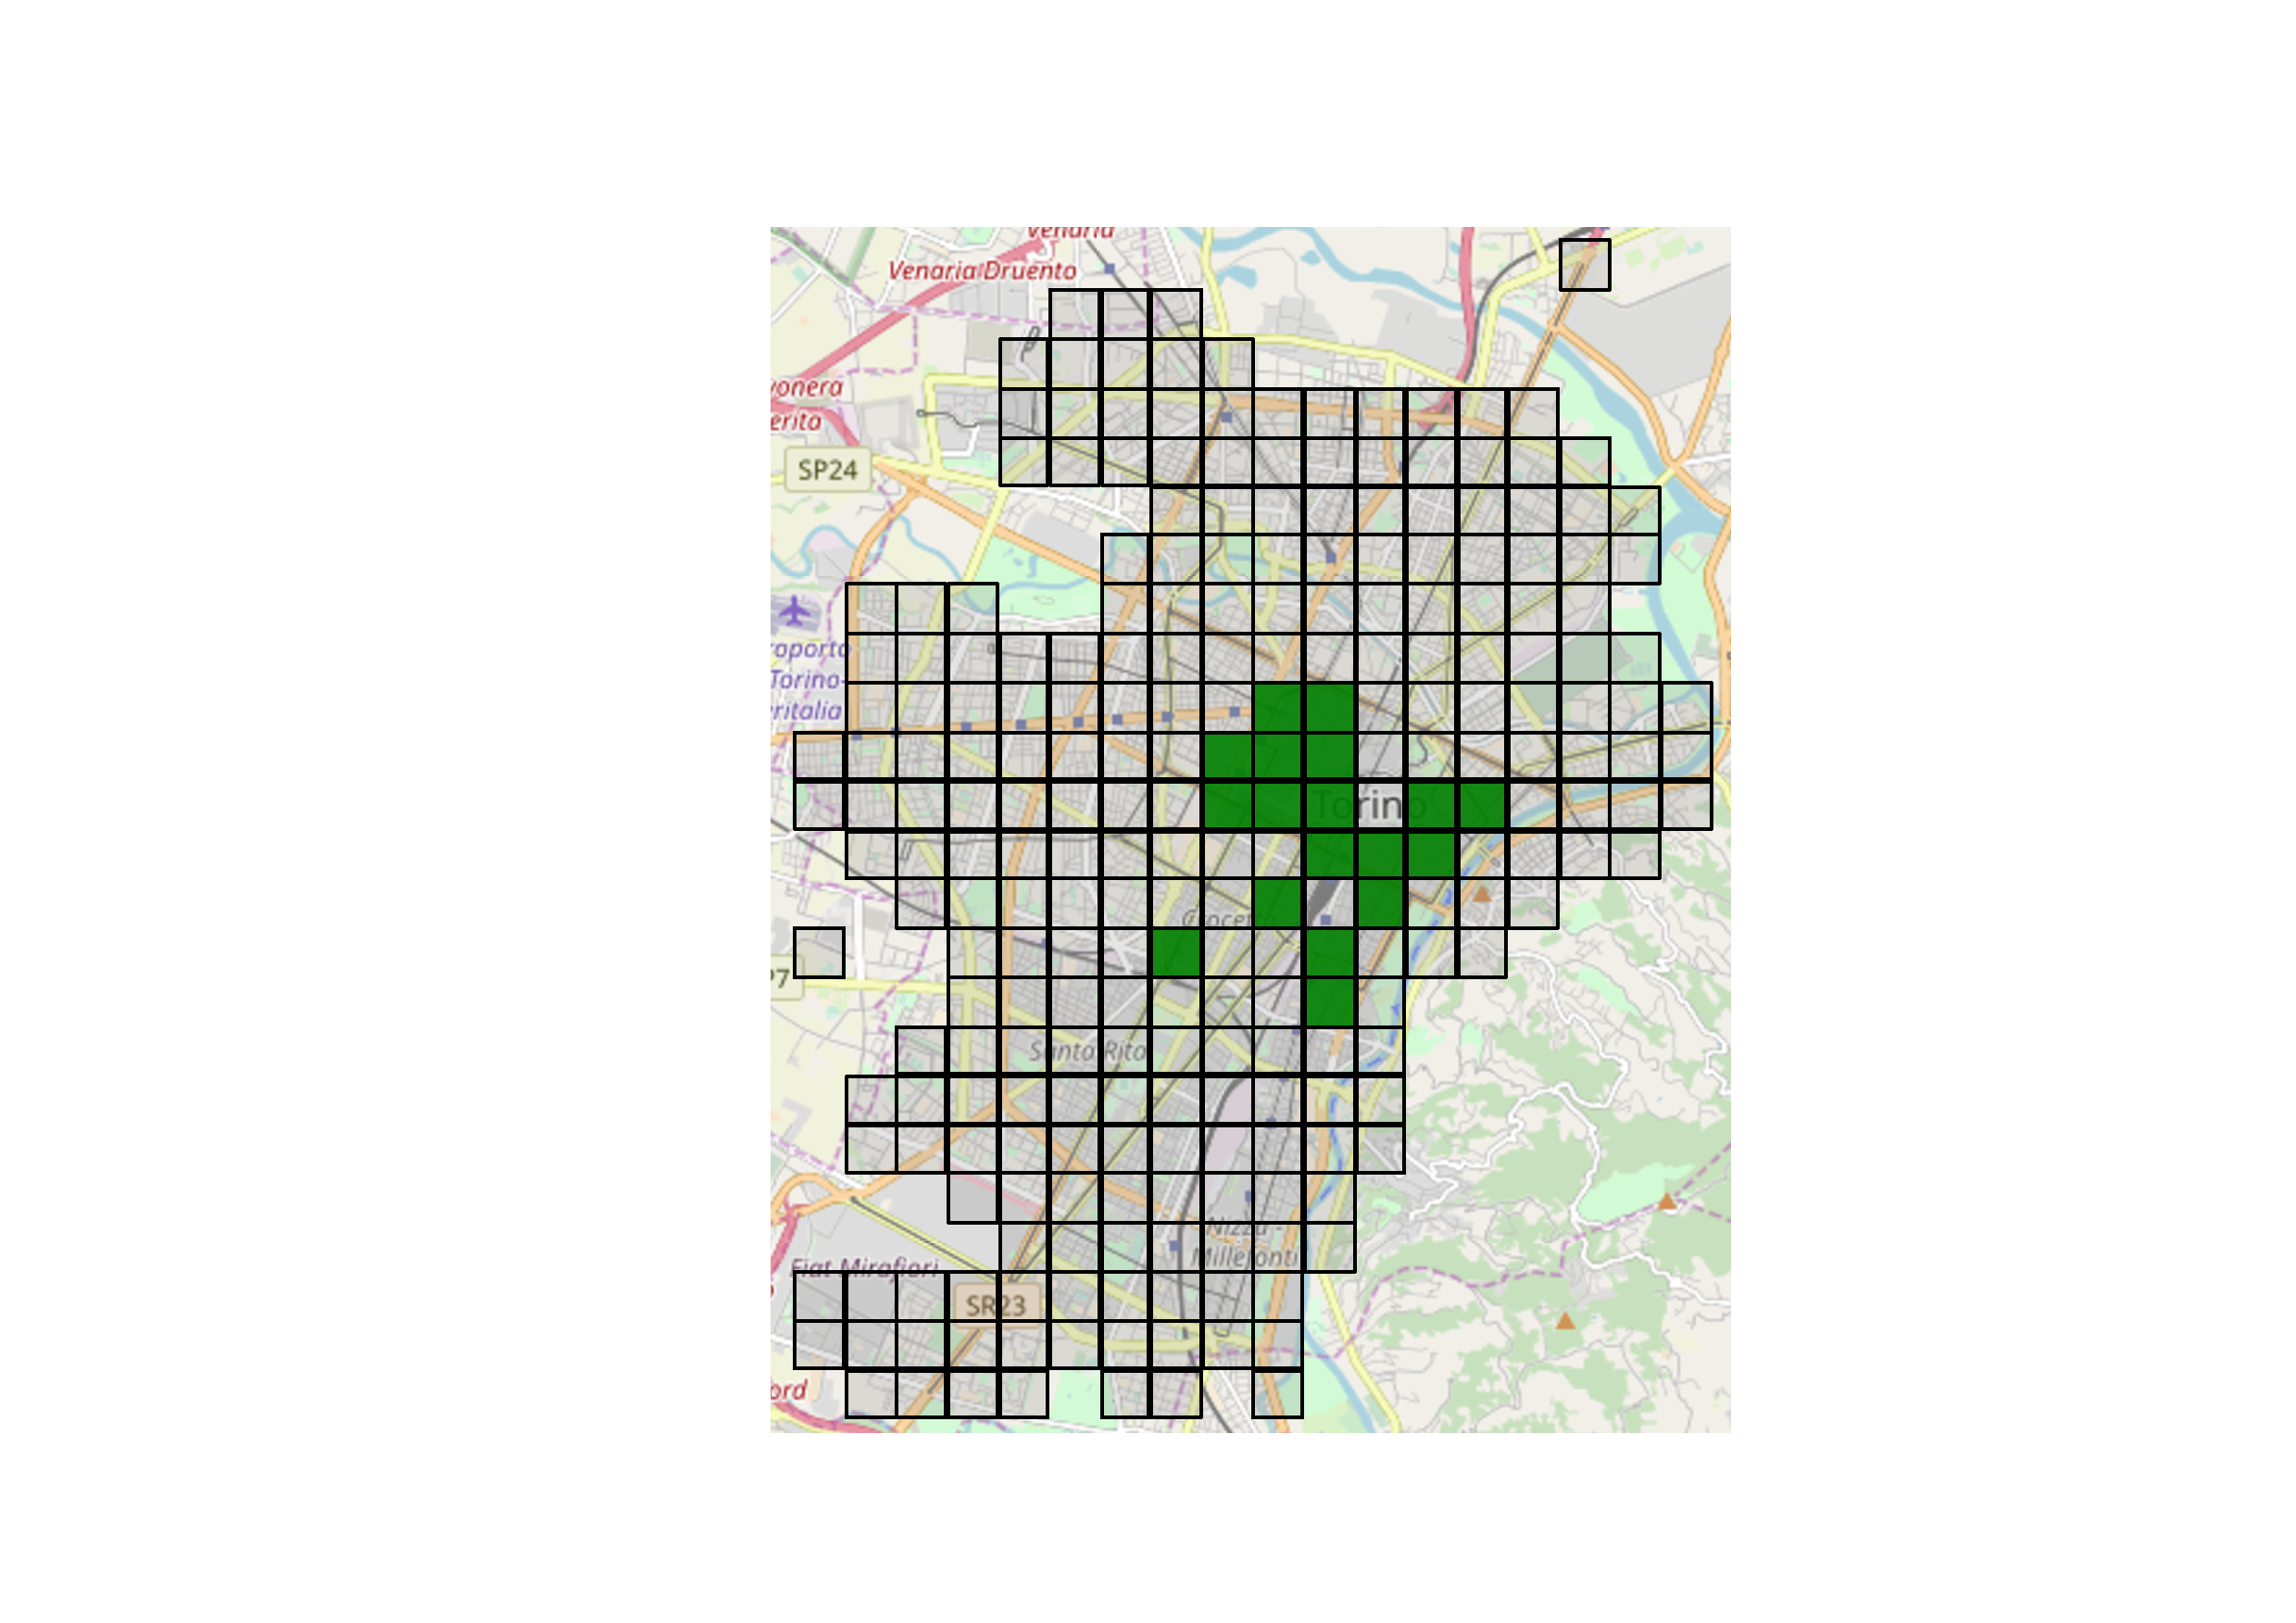
\includegraphics[width=0.3\columnwidth]{figures/NP_hybrid_18_Torino_placement.pdf}
        \label{fig:7_7a_hm_max-parking_3}
    }
    \subfloat[][\textit{Local Search}.]
    {
        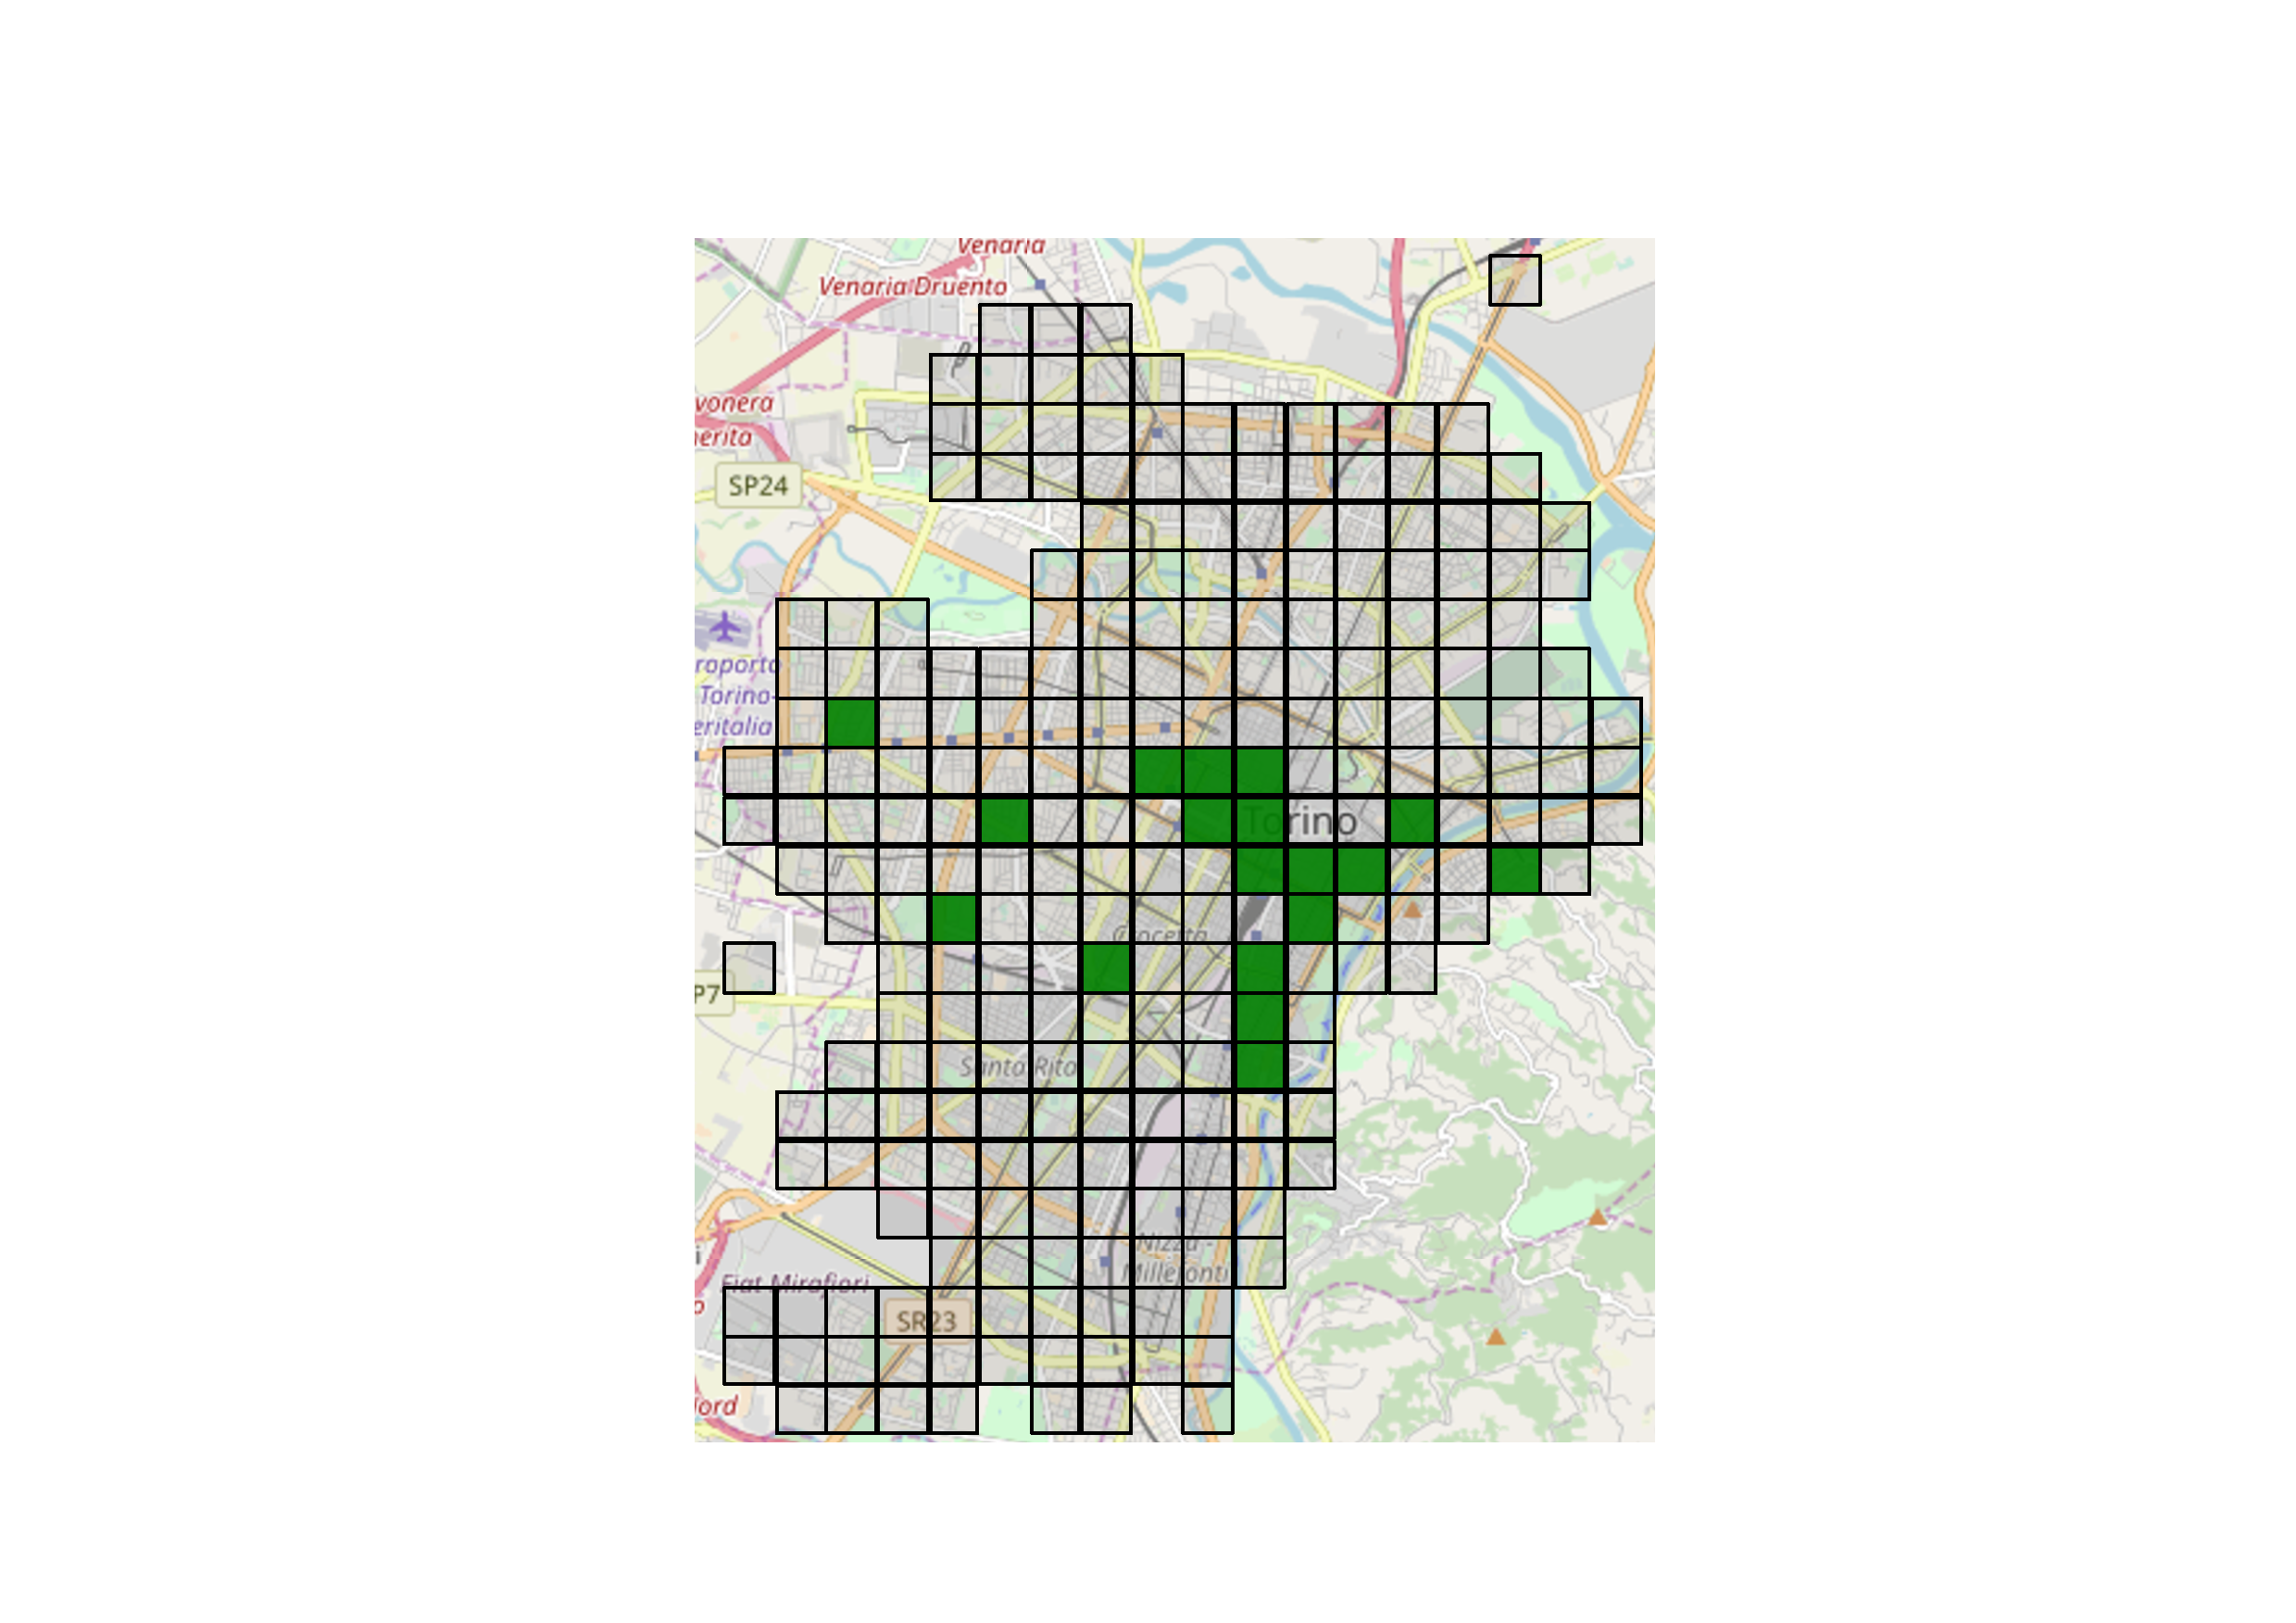
\includegraphics[width=0.3\columnwidth]{figures/LS_hybrid_18_Torino_placement.pdf}
        \label{fig:7_7a_hm_local3}
    }
    \subfloat[][\textit{Genetic} algorithm.]
    {
        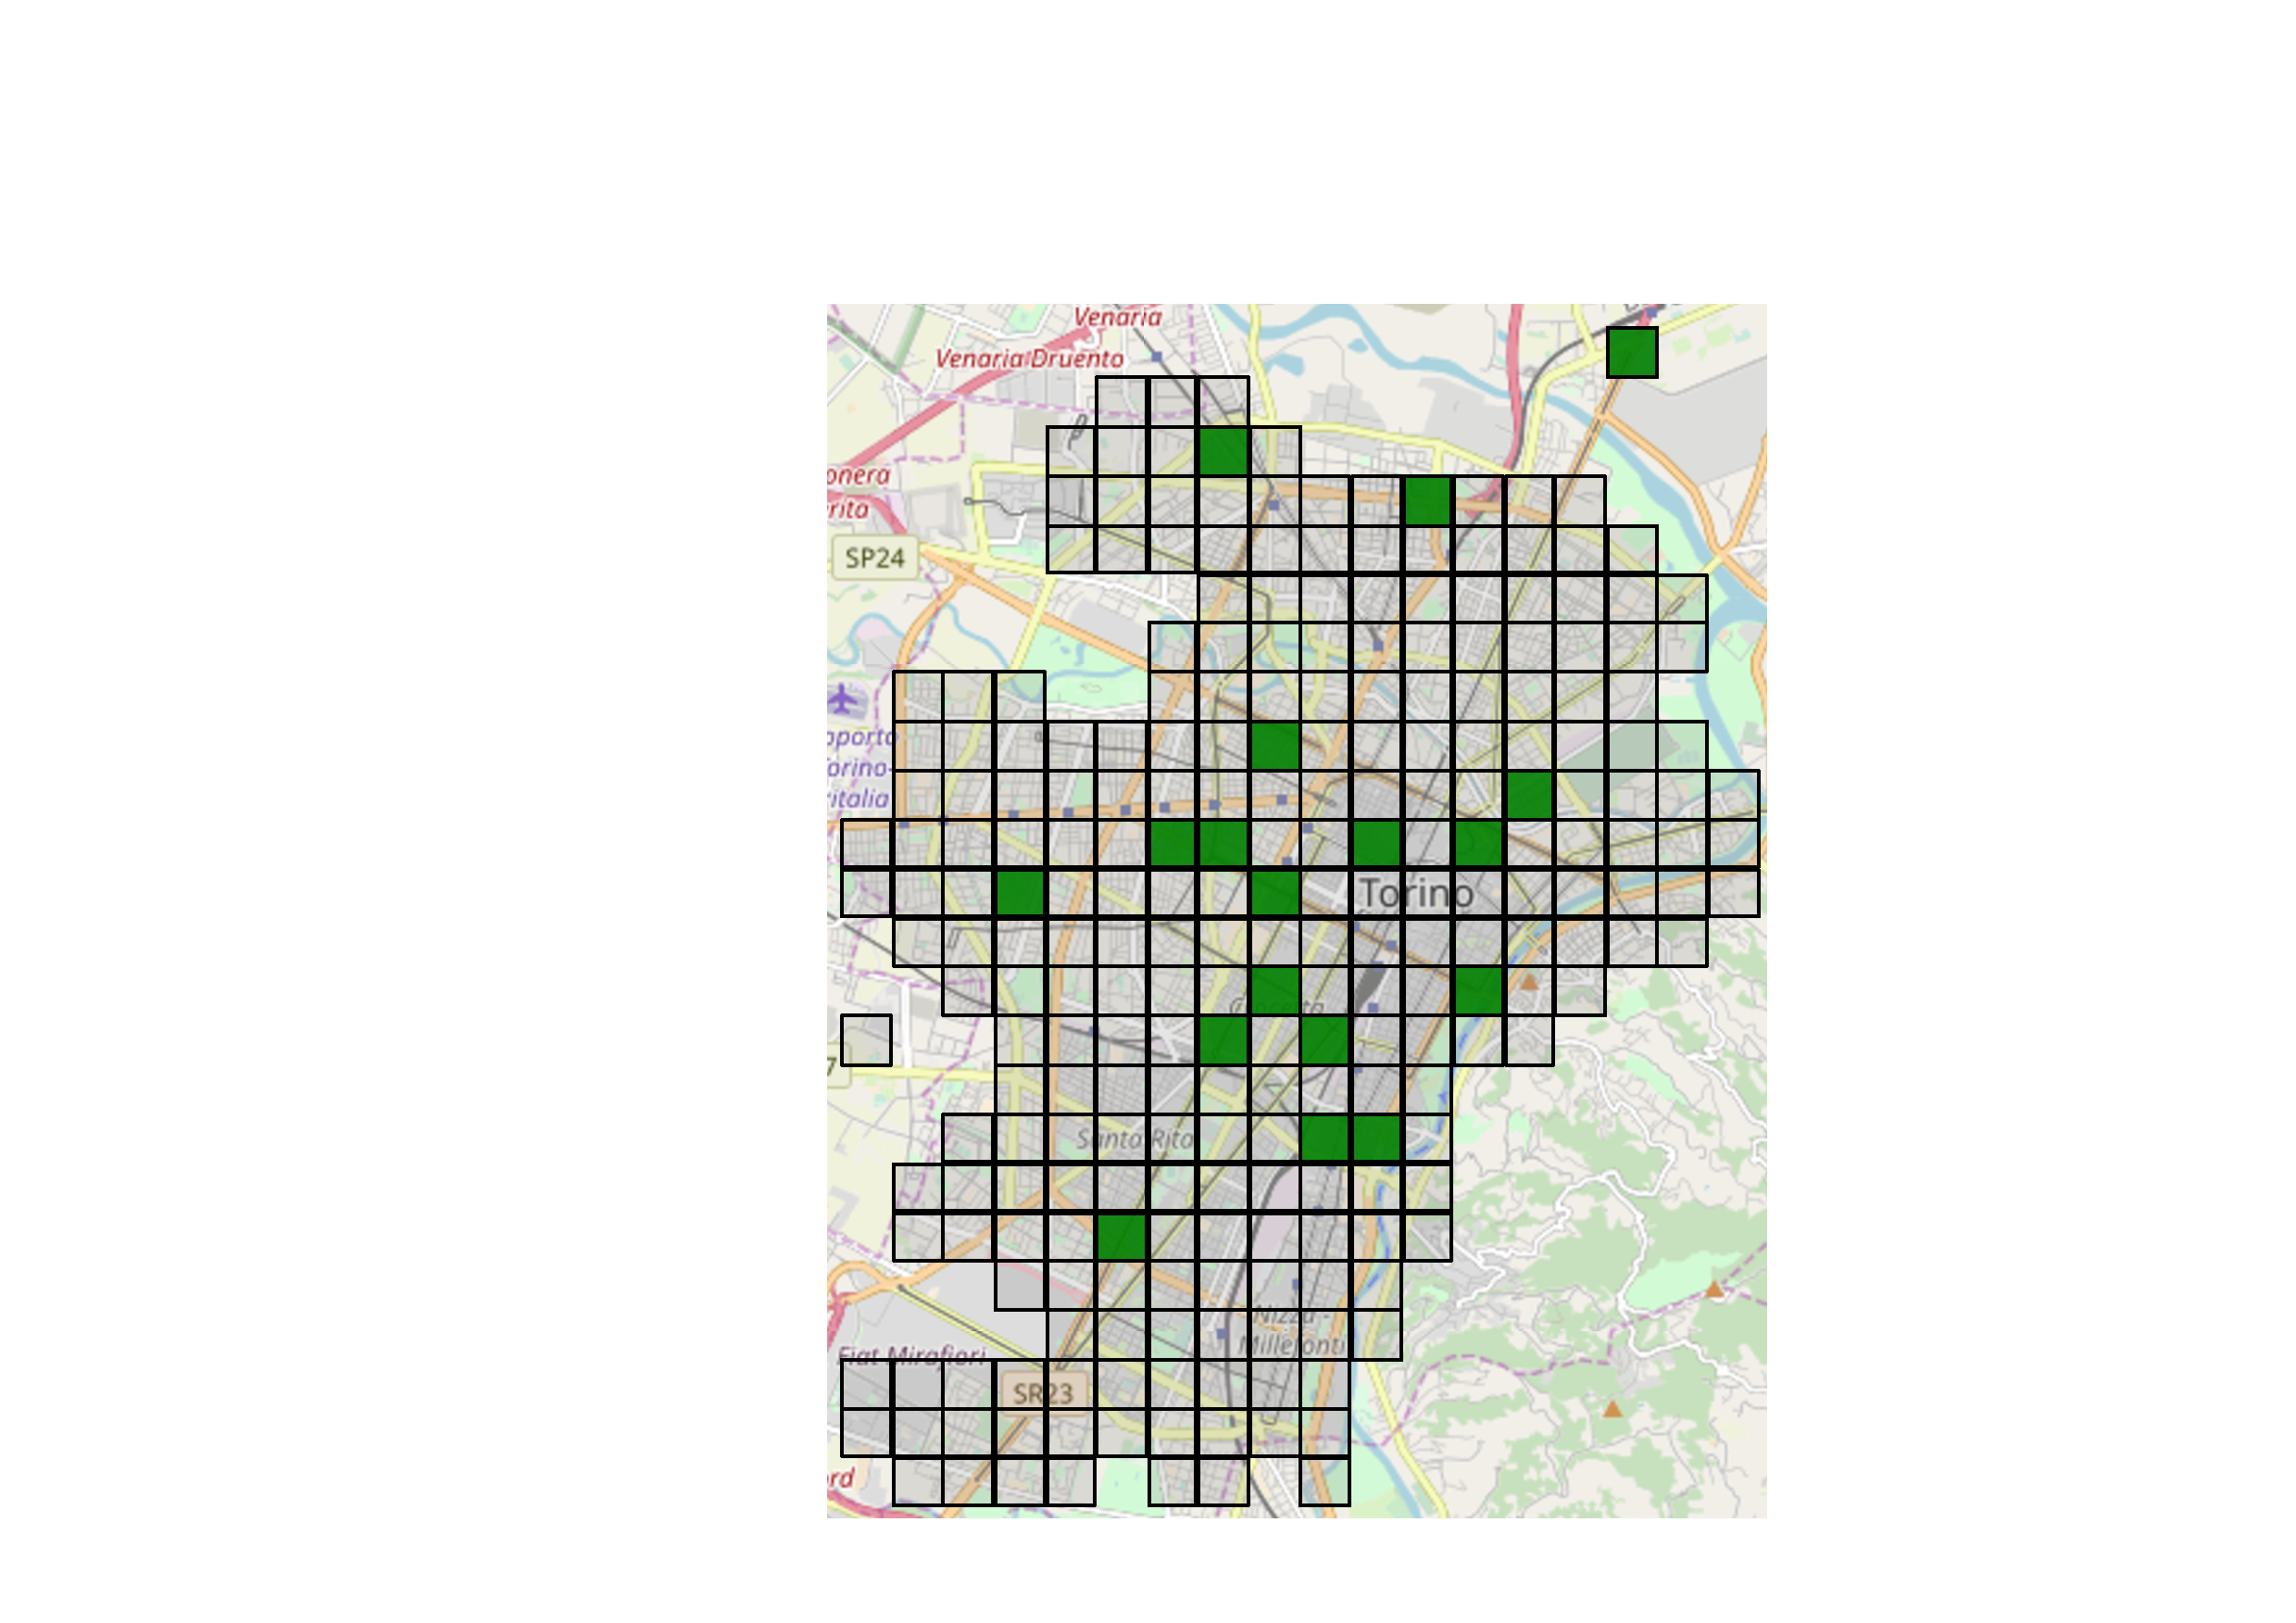
\includegraphics[width=0.3\columnwidth]{figures/GN_hybrid_18_Torino_placement.pdf}
        \label{fig:7_7a_hm_genetico3}
    }
    \caption{Different placement of 18 zones (7\% of the total) for (a) Number of parkings per zone, (b) \textit{Local Search}  and (c) \textit{Genetic} solution. Darker areas have larger values.}
    \label{fig:7_7a_maps}
\end{figure}

To give a feeling about the differences in the solutions found by different algorithms, figure.~\ref{fig:7_7a_maps} reports the solutions obtained with 7\% of the zones equipped with charging stations (i.e., $Z=18$ zones).   

\textit{Num parking} solution, figure~\ref{fig:7_7a_hm_max-parking_3}, places most of the charging stations in downtown area and near the main train stations. 
\textit{Local Search}, figure~\ref{fig:7_7a_hm_local3}, still has many zones in common with \textit{Num parking}, the solution it started from. It just spreads some charging station to cover also some remote zones.
The \textit{Genetic} algorithm, figure.~\ref{fig:7_7a_hm_genetico3}, shows very few zones in common with \textit{Num parking}. Charging stations are spread all over the city, still with more density in the city centre. 
 

\subsection{Validation of optimised configurations}

\begin{figure}[t]
    \centering     %%% not \center
    \subfloat[][Percentage of infeasible trips. Y-Axis is logarithmic.]
    {
        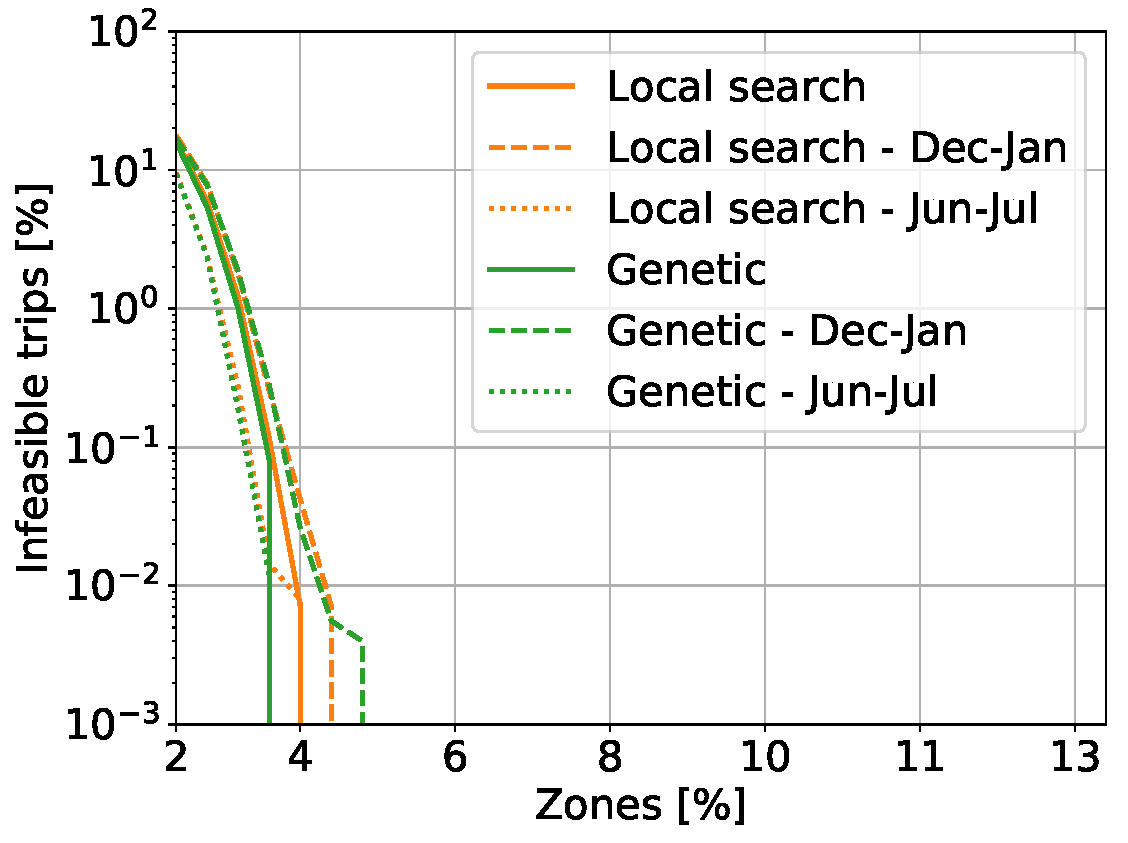
\includegraphics[width=0.45\columnwidth]{figures/Deaths_comparison.pdf}
        \label{fig:7_7a_inf_validation}
    }
    \subfloat[][Walked distance, averaged over all trips.]
    {
        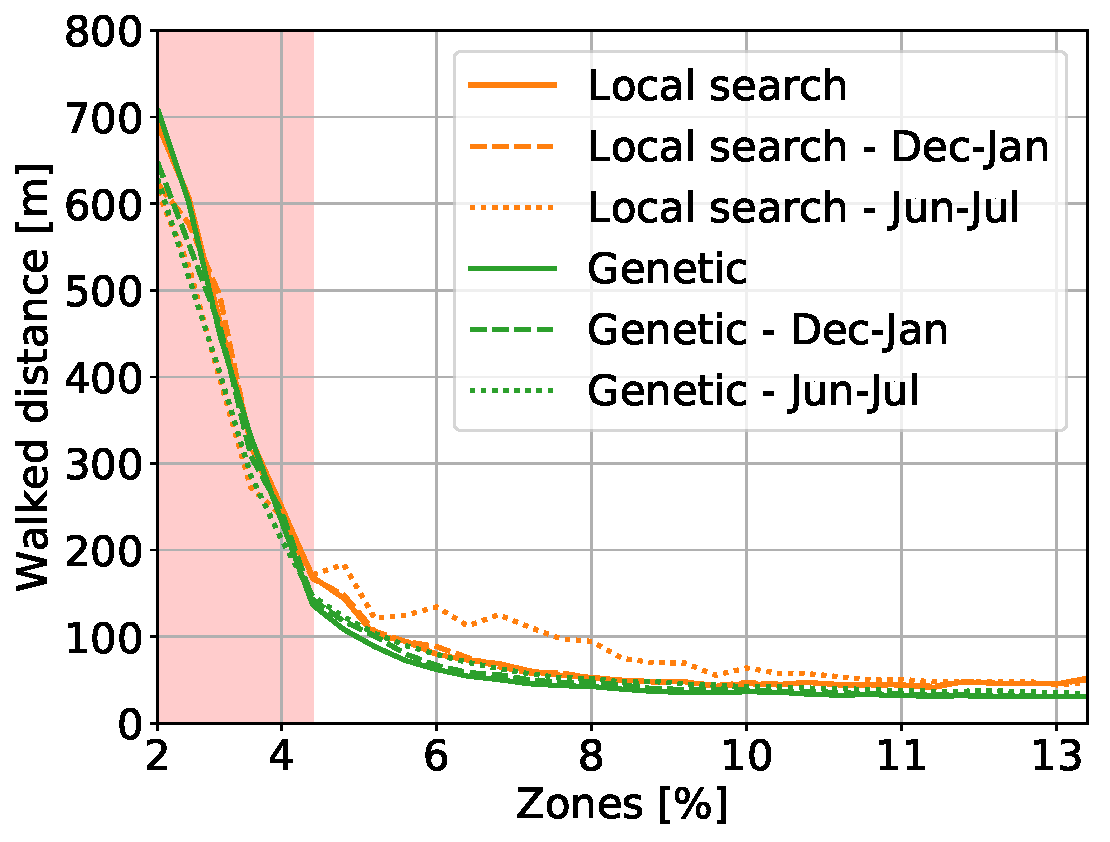
\includegraphics[width=0.45\columnwidth]{figures/TravelWithPenlaty_comparison.pdf}
        \label{fig:7_7a_walked_validation}
    }

    \caption{Performance of the optimised configuration, tested on other 2 months long data-sets.}
    \label{fig:validation}
\end{figure}

The optimised solutions presented in the previous section are built through data-driven simulations. Hence they might over-fit the data of the specific considered period and not be robust to customers' habit changes. To validate those findings, I test the output placement configurations by using independent test traces, different from the one used to run the optimisation. 
I rely on two traces collected in Turin in two different periods of the year: one in summer, from June to July 2017; the other in winter, from December 2017 to January 2018. I focus on these two periods since in summer and near Christmas holidays the users may exhibit different habits (e.g., customers may rent the cars to go to parks and swimming pools during summer). These anomalies may represent a challenge for the optimised configurations.
In the summer trace I record about  100\,000 rentals, while in the winter one 128\,000 rentals (respectively 8\% less and 3\% more with respect to the September/October trace). I compute the best station placement considering the September and October 2017 trace, and test system performance using the summer and winter traces.  

Figure~\ref{fig:validation} compares results. I consider both \textit{Local Search} and \textit{Genetic} algorithms.
In almost all cases, differences are negligible, showing that the solution is robust. For example, for 13\% of zones and considering \textit{Genetic} algorithm, the walked distance on the tests are just 2\,m above those in the trace used for optimisation. Notice how in June and July the \textit{Local Search} behaves worse than other cases: this is possibly due to the different mobility patterns in summer, while the Local Search solution could still be too related to the number of parkings in September-October. On the other hand, the solution found by the global genetic algorithm is robust.
